\section{Introduction}
\begin{figure}
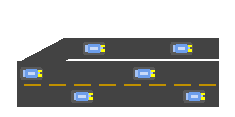
\includegraphics[scale=2]{figures/frontage.pdf}
\caption{Motivating Example: Differentiating vehicles on nearby parallel roads}
\label{fig:frontage}
\end{figure}

Many systems today keep track of objects in real-time through positioning technologies such as the satelite Global Positioning System~(GPS)\cite{gpsGov}.
However, positioning technologies have inherent error, which can range from centimeters to tens of meters.
Consider the issue of tracking the number of vehicles exiting a highway to an adjacent, parallel frontage road (\figref{fig:frontage}). All vehicles are still going in the same direction, at similar speeds. The difference in relative position could easily be within the error of GPS under poor conditions.

This problem can be handled in a number of different ways. If additional sensors can be used, then disparate information can be combined to produce more accurate results, known as \textit{sensor fusion}~\cite{moravecAIM88}.
Alternatively, historical sensor information can be used to refine new sensor inputs.
Finally, rules can be introduced to help clean up random information. Returning to our example, if the vehicle velocity drops below highway speeds over a period of time, it could be assumed to have left the faster roadway.

This work combines historical information with probablistic rules, using techniques similar to sensor fusion to combine continuous probabilities. Continuous probability spaces of position and velocity are approximated with 4-dimensional meshes, which can be efficiently combined to refine location estimates.
